% $Header: /home/vedranm/bitbucket/beamer/solutions/generic-talks/generic-ornate-15min-45min.en.tex,v 90e850259b8b 2007/01/28 20:48:30 tantau $

\documentclass{beamer}

% This file is a solution template for:

% - Giving a talk on some subject.
% - The talk is between 15min and 45min long.
% - Style is ornate.



% Copyright 2004 by Till Tantau <tantau@users.sourceforge.net>.
%
% In principle, this file can be redistributed and/or modified under
% the terms of the GNU Public License, version 2.
%
% However, this file is supposed to be a template to be modified
% for your own needs. For this reason, if you use this file as a
% template and not specifically distribute it as part of a another
% package/program, I grant the extra permission to freely copy and
% modify this file as you see fit and even to delete this copyright
% notice. 


\mode<presentation>
{
  \usetheme[secheader]{Boadilla}
  %\usetheme{Warsaw}
  % or ...

  \setbeamercovered{transparent}
  % or whatever (possibly just delete it)
}


\usepackage{graphicx}
\graphicspath{{fig/}}
\usepackage{listings}
\usepackage{xspace}
\usepackage{amsmath}
\usepackage{fontspec,xunicode,xltxtra}
\usepackage[slantfont,boldfont]{xeCJK} % 允许斜体和粗体

\setCJKmainfont[BoldFont={WenQuanYi Zen Hei},
%ItalicFont={AR PL UKai CN}]{AR PL UMing CN}
ItalicFont={AR PL UKai CN}]{WenQuanYi Micro Hei}
\setCJKsansfont{WenQuanYi Zen Hei}
\setCJKmonofont{WenQuanYi Zen Hei Mono}

\setCJKfamilyfont{zhsong}{AR PL UMing CN}
\setCJKfamilyfont{zhhei}{WenQuanYi Zen Hei}
\setCJKfamilyfont{zhkai}{AR PL UKai CN}

\newcommand*{\songti}{\CJKfamily{zhsong}} % 宋体
\newcommand*{\heiti}{\CJKfamily{zhhei}}   % 黑体
\newcommand*{\kaishu}{\CJKfamily{zhkai}}  % 楷书

\setmainfont{TeX Gyre Pagella} % 英文衬线字体
%\setmonofont{Microsoft YaHei} % 英文等宽字体
%\setsansfont{Trebuchet MS} % 英文无衬线字体

% fix: navi button not working with XeTeX
% SEE: http://bbs.ctex.org/viewthread.php?tid=64104
\makeatletter
\def\beamer@linkspace#1{%
  \begin{pgfpicture}{0pt}{-1.5pt}{#1}{5.5pt}
    \pgfsetfillopacity{0}
    \pgftext[x=0pt,y=-1.5pt]{.}
    \pgftext[x=#1,y=5.5pt]{.}
  \end{pgfpicture}}
\makeatother

\def\TeXLive{\TeX{} Live\xspace}
\let\TL=\TeXLive
\title % (optional, use only with long paper titles)
{Fedora and \TL}

\author[alick] % (optional, use only with lots of authors)
{Alick Zhao\inst{1}}
% - Use the \inst{?} command only if the authors have different
%   affiliation.

\institute[Tsinghua University] % (optional, but mostly needed)
{
  %\inst{1}%
  \texttt{alick9188@gmail.com}\\
  Department of Electronic Engineering\\
  Tsinghua University
}
% - Use the \inst command only if there are several affiliations.
% - Keep it simple, no one is interested in your street address.

\date[FAD Beijing 2011] % (optional)
{Oct 15, 2011 / FAD Beijing 2011}

\subject{Talks, TeX Live, FAD, Fedora}
% This is only inserted into the PDF information catalog. Can be left
% out. 

% If you have a file called "university-logo-filename.xxx", where xxx
% is a graphic format that can be processed by latex or pdflatex,
% resp., then you can add a logo as follows:

% \pgfdeclareimage[height=0.5cm]{university-logo}{university-logo-filename}
% \logo{\pgfuseimage{university-logo}}



% Delete this, if you do not want the table of contents to pop up at
% the beginning of each subsection:
\AtBeginSubsection[]
{
  \begin{frame}<beamer>{Outline}
    \tableofcontents[currentsection,currentsubsection]
  \end{frame}
}


% If you wish to uncover everything in a step-wise fashion, uncomment
% the following command: 

%\beamerdefaultoverlayspecification{<+->}

\lstset{basicstyle=\ttfamily,breaklines=true}
\hypersetup{
%colorlinks=true,
%pdfpagemode=FullScreen,
}

\begin{document}

\begin{frame}
  \titlepage
\end{frame}

\begin{frame}{Outline}
  \tableofcontents
  % You might wish to add the option [pausesections]
\end{frame}


% Since this a solution template for a generic talk, very little can
% be said about how it should be structured. However, the talk length
% of between 15min and 45min and the theme suggest that you stick to
% the following rules:  

% - Exactly two or three sections (other than the summary).
% - At *most* three subsections per section.
% - Talk about 30s to 2min per frame. So there should be between about
%   15 and 30 frames, all told.

\section{Introduction}

\subsection{\TeX}

\begin{frame}{What is \TeX ?}
  % - A title should summarize the slide in an understandable fashion
  %   for anyone how does not follow everything on the slide itself.

  \begin{itemize}
    \item a typysetting system for beautiful books
    \item developed by Donald E.~Knuth in 1980s
    \item free to use, free to modify with naming exception
    \item \TeX\ 3.1415926 as of 2011
  \end{itemize}
\end{frame}

\begin{frame}{Why \TeX ?}
  \begin{itemize}
    \item excel in typesetting math formular (\AmS-\TeX{})
    \item allow the author to focus on the content without bothering the
      layout
    \item enhanced in many aspects
      \begin{itemize}
        \item Chinese
        \item slides (Beamer)
        \item music notes, chess, etc
      \end{itemize}
  \end{itemize}
\end{frame}

%\begin{frame}{Make Titles Informative.}
%
  %You can create overlays\dots
  %\begin{itemize}
  %\item using the \texttt{pause} command:
    %\begin{itemize}
    %\item
      %First item.
      %\pause
    %\item    
      %Second item.
    %\end{itemize}
  %\item
    %using overlay specifications:
    %\begin{itemize}
    %\item<3->
      %First item.
    %\item<4->
      %Second item.
    %\end{itemize}
  %\item
    %using the general \texttt{uncover} command:
    %\begin{itemize}
      %\uncover<5->{\item
        %First item.}
      %\uncover<6->{\item
        %Second item.}
    %\end{itemize}
  %\end{itemize}
%\end{frame}

\begin{frame}{An overview of \TeX\ system}
  \begin{itemize}
    \item Formats: Plain \TeX, \LaTeX, \AmS-\TeX, Con\TeX{}t
    \item Engines: tex, latex, pdf(la)tex, xe(la)tex, lua(la)tex
    %\item utils: dvips, xdvipdfmx, 
      \pause
    \item Distros: \TL, MiKTeX, MacTeX
  \end{itemize}
\end{frame}

\subsection{\TeXLive}

\begin{frame}{What is \TL ?}
  \begin{itemize}
    \item a \TeX\ distro: a comprehensive collection of \TeX\ utils
    \item developed since 1996 by collaboration between TeX user groups
    \item originally for Linux, now cross-platform
    \item can run live from a DVD (up to v2009)
    \item default TeX distro for Fedora, Ubuntu, Debian, Gentoo
  \end{itemize}
\end{frame}

\section{Install \TL}
\subsection{local version}
\begin{frame}{Methods}
  \begin{itemize}
    \item download the huge DVD iso
    \item be a member of TUG and get \TL on DVD
      \pause
    \item net install
  \end{itemize}
\end{frame}

\begin{frame}[fragile]
  \frametitle{网络安装}
  \begin{itemize}
    \item 
从 \TeXLive 镜像下载
install-tl-unx.tar.gz
和
install-tl-unx.tar.gz.sha256
\begin{itemize} % several mirror url
  \item \url{http://mirrors.tuna.tsinghua.edu.cn/CTAN/systems/texlive/tlnet/}
  \item \url{http://ftp.ctex.org/mirrors/CTAN/systems/texlive/tlnet/}
  \item Check \url{http://mirror.ctan.org/README.mirrors}
\end{itemize}

\item 校验
\begin{lstlisting}
$ LANG=C sha256sum --check install-tl-unx.tar.gz.sha256 
install-tl-unx.tar.gz: OK
\end{lstlisting}

  \end{itemize}
\end{frame}

\begin{frame}[fragile]
  \frametitle{网络安装}
  \begin{itemize}
    \item 安装
      \begin{lstlisting}
su -c'./install-tl -gui -repository http://mirrors.tuna.tsinghua.edu.cn/CTAN/systems/texlive/tlnet/'
      \end{lstlisting}

(图形界面需要 Perl Tk 模块,可能还需要 xhost +)

\item 截图
\end{itemize}
\end{frame}

\begin{frame}
  \begin{figure}[h]
  \centering
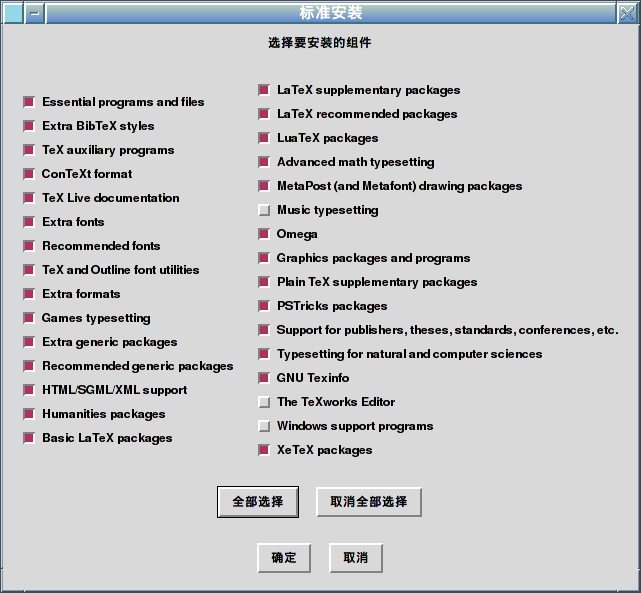
\includegraphics[scale=0.45]{标准安装.png}
  \end{figure}
\end{frame}

\begin{frame}
  \begin{figure}[h]
  \centering
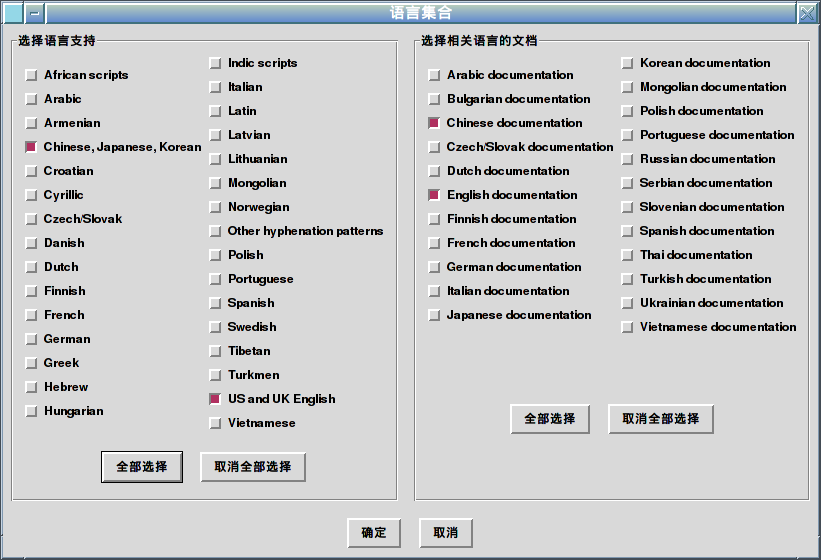
\includegraphics[scale=0.4]{语言集合.png}
  \end{figure}
\end{frame}

\begin{frame}
  \begin{figure}[h]
  \centering
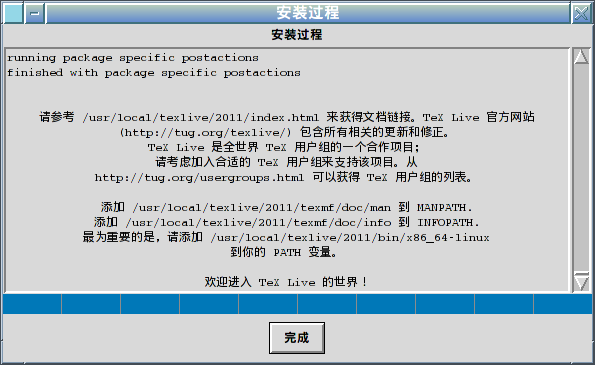
\includegraphics[scale=0.5]{安装过程.png}
  \end{figure}
\end{frame}

\begin{frame}[fragile]
  \frametitle{网络安装后配置}
\begin{itemize}
  \item 
打开 \TeXLive 指南中文版 ``texlive-zh-cn.pdf'',
关注第 3.4 节
  \begin{lstlisting}
texdoc texlive-zh
  \end{lstlisting}

  \item 
    Add the following lines into your \nolinkurl{~/.bash_profile}:
    \begin{lstlisting}
export PATH=/usr/local/texlive/2011/bin/x86_64-linux:$PATH
export MANPATH=/usr/local/texlive/2011/texmf/doc/man:$MANPATH
export INFOPATH=/usr/local/texlive/2011/texmf/doc/info:$INFOPATH
    \end{lstlisting}

\end{itemize}
\end{frame}

\begin{frame}[fragile]
  \frametitle{网络安装后配置}
  \begin{itemize}
\item
\XeTeX\ and fontconfig:
\begin{lstlisting}
# cp /usr/local/texlive/2011/texmf-var/fonts/conf/texlive-fontconfig.conf /etc/fonts/conf.d/09-texlive.conf
# fc-cache -fsv
\end{lstlisting}

\item Con\TeX{}t Mark IV
  \begin{lstlisting}
context --generate
  \end{lstlisting}

\end{itemize}
\end{frame}

\lstdefinestyle{latex}{
language={[LaTeX]TeX},
frame=single,
escapeinside=``,
keywordstyle=\color{red!70},
}

\begin{frame}[fragile]
  \frametitle{网络安装后测试}
  \begin{itemize}
    \item 
  \begin{lstlisting}
latex sample2e.tex
xdvi sample2e.dvi
xetex opentype-info.tex
  \end{lstlisting}

\item 编写文件 ``test-chinese.tex''
  \begin{lstlisting}[style=latex]
\documentclass{ctexart}
\setCJKmainfont{WenQuanYi Zen Hei}
\begin{document}
\TeX{}`你好!`
\end{document}
  \end{lstlisting}
  编译得到 PDF 文档
  \begin{lstlisting}
xelatex test-chinese
evince test-chinese.pdf
  \end{lstlisting}

  \end{itemize}
\end{frame}

\subsection{sys version/ rpm}
%texlive 2007 :(

% TeX Live in Linux distro repo
% Ubuntu: as of July 2011 the texlive package that ships with Ubuntu
% (TeX Live 2009) is lagging two years behind the current TeX Live
% release (TeX Live 2011). (https://help.ubuntu.com/community/LaTeX)
\begin{frame}
  \begin{table}[htbp]
	\centering
	\caption{调查结果}
	\begin{tabular}{lllp{6em}}
		\hline
版本		&仓库	&安装方式/发行版&体验\\
		\hline
2011		&CTAN	&ISO(BT)	&强大 \\
2011		&distro	&Gentoo Portage	&少许问题 \\
2011		&CTAN	&net		&Debian sid 刚用不久 \\
2010,2011	&?	&?		&Debian 很好 \\
2010		&CTAN	&net		&XP+Linux 挺好除了不能滚动升级 \\
2007		&distro	&Fedora 15	&xetex 挺好 \\
2009		&distro	&Ubuntu 10.04	&已有xecjk \\
2011		&CTAN	&net		&不错 \\
2009		&distro	&Ubuntu 11.04	&xelatex \\
		\hline
	\end{tabular}
	\label{tab:poll_result}
\end{table}


\end{frame}

\begin{frame}
  \frametitle{\TL in Linux distros}
  \begin{itemize}
    \item Fedora offical repo: \TL 2007 \hfill Not good.
    \item Ubuntu offical repo: \TL 2009 \hfill Not good.
    \item jnovy's repo \TL 2010\&2011 \hfill Good news.

      \url{http://fedoraproject.org/wiki/Features/TeXLive}
  \end{itemize}
\end{frame}

% jnovy's repo 2011
% wiki page
\begin{frame}[fragile]
  \frametitle{安装步骤}
  
\begin{lstlisting}
# rpm -i http://jnovy.fedorapeople.org/texlive/packages.f14/texlive-release.noarch.rpm
# yum clean all
# yum install texlive
\end{lstlisting}
Then you get basic \TL scheme.
(yum install texlive-scheme-full, if space is not an issue.)

\begin{lstlisting}
yum install texlive-collection-xetex texlive-ctex
yum install 'tex(savesym.sty)'
yum install 'tex(siunitx.sty)'
\end{lstlisting}

\begin{lstlisting}
xelatex template-xetex.tex
\end{lstlisting}

\end{frame}

\begin{frame}{Why rpm?}
  \begin{itemize}
    \item single installation tool
    \item package dependency
    \item no old packages in \TL repo
  \end{itemize}
\end{frame}

\section{Use \TL}

\begin{frame}{Help Yourself}
  \begin{itemize}
    \item tlmgr (Yum in Fedora version)
      \begin{itemize}
        \item \texttt{tlmgr gui}
        \item \texttt{man tlmgr}
      \end{itemize}

    \item texdoc (may need yum install)
      \begin{itemize}
        \item e.g. \texttt{texdoc xecjk},
          \texttt{texdoc mathmode}, and \texttt{texdoc symbols}
        \item \texttt{texdoctk} --- GUI
      \end{itemize}
  \end{itemize}
\end{frame}

\begin{frame}{\TeX\ community}
  \begin{itemize}
    \item BBS
      \begin{itemize}
        \item smth TeX board
        \item bbs.ctex.org
      \end{itemize}
    \item Mailing list
      \begin{itemize}
        \item \TL: \url{http://tug.org/mailman/listinfo/tex-live}
        \item Fedora: \url{http://www.linux.cz/pipermail/texlive/}
      \end{itemize}
    \item uk FAQ: \url{http://www.tex.ac.uk/cgi-bin/texfaq2html}
    \item google
  \end{itemize}
\end{frame}

\begin{frame}{General Tips}
  \begin{itemize}
    \item focus on the content, not the layout
      (use well-defined classes/templates: ctexart, beamer, thuthesis)
    \item TeX Editor? (Vim, Emacs, LyX, TeX IDE\dots)
    \item \texttt{texcount -ch report.tex}: count words
    \item Makefile
  \end{itemize}
\end{frame}

\section*{Summary}

\begin{frame}{Summary}

  % Keep the summary *very short*.
  \begin{itemize}
  \item \TL makes typesetting easy.
  \item The installation of \TL is easy.
  \item Happy \LaTeX{}ing!
  \end{itemize}
  
  % The following outlook is optional.
  \vskip0pt plus.5fill
  \begin{itemize}
  \item
    Outlook
    \begin{itemize}
    \item
      Vim LaTeX suite
    \item
      Show the procedure of using \TeX?
    \end{itemize}
  \end{itemize}
\end{frame}

\section*{Appendix}

\begin{frame}
  \begin{itemize}
    \item Get these materials from \alert{github}
      \begin{itemize}
          % FIXME
        \item templates: \url{http://github.com/alick9188/TeXLab}
        \item FAD slides: \url{http://github.com/alick9188/fad-texlive-talk}
      \end{itemize}
    \item License: CC-BY-SA
  \end{itemize}
\end{frame}

\begin{frame}
  \begin{center}
    \Large
  Thanks!

  Q\&A
\end{center}
\end{frame}

\end{document}
%%% vim: set sw=2 isk+=\: et tw=70 formatoptions+=mM:
